\section{Integrity-Protected State}
\label{sec:integrity-state}

This section introduces the storage model on which the architecture rests. Any party holding a commitment can verify data against it, even when it holds only part of that data. \Cref{sec:history-entanglement,sec:self-encoding,sec:journal-web} each build on this model.

\subsection{The Value of Verifiable State}

Versioned systems preserve the path by which information changed. Git turns a working tree into a succession of content-addressed snapshots, append-only databases and blockchains bind later entries to earlier ones, and transparency systems publish authenticated views that clients and witnesses can compare~\cite{Haber1991timestamp,Laurie2014certificate,Melara2015coniks}. Their common achievement is to establish whether the evidence now presented belongs to the state that was previously committed. That answer changes the character of a \glslink{record}{record}. A mutable database row can only be read by asking the operator for its current value, whereas a committed state can also be held by a recipient, cited by \glslink{digest}{digest}, compared with another copy, and revisited after the operator changes its presentation. Recipients can preserve history alongside the service as portable evidence. This property remains valuable even when the record is incomplete, disputed, or false, because \glslink{integrity}{integrity} preserves the subject of later analysis rather than vouching for its truth.

Authenticated data structures typically deliver these guarantees through queries, in which a verifier receives a query result and a compact proof against a known root~\cite{Martel2004general,Miller2014authenticated}. This paper calls the property of being checkable against a commitment \emph{integrity-verifiable} and reserves \glslink{authentication}{authentication} for identity, origin, and authority, keeping digest consistency, signatures, and authorization visible as separate checks. The \glslink{synchronic-web}{Synchronic Web} departs from this query-and-proof model by making partial knowledge persistent, so that a recipient can retain one region of a state, discard another, and later combine compatible evidence while referring throughout to the same logical commitment. That capability begins with a deliberately small structural model.

\subsection{A Minimal Verifiable Structure}
\label{sec:minimal-structure}

The native substrate is an integrity-verifiable binary data-structure DAG in which immutable substructures may be shared by many parents. Uniform two-child nodes keep identifier derivation, slicing, and proofs the same everywhere, and richer structures such as maps and chains are built from them above the substrate. A \emph{logical digest} names recursively defined content or structure, while a \emph{node identifier} retrieves the representation available in one store. The separation matters because identity and storage answer different questions. The same logical state may use different persistence layouts, and one store may hold either complete structure or a compact record of its digest. A root is a \emph{durable handle}, a stable local name that maps to the node identifier of the current state, and branches, leaves, \glslink{stump}{stumps}, and null describe the structure reachable from a root. These concepts support maps, \glslink{object}{objects}, histories, and \glslink{resource}{resources}, as shown in \cref{fig:dag-stump}:

\begin{itemize}
  \item \textbf{Root:} a durable handle mapped to a \glslink{node}{node} identifier.
  \item \textbf{Branch:} two child node identifiers with a logical digest derived from their digests.
  \item \textbf{Leaf:} raw content bound into the structure by its digest.
  \item \textbf{Stump:} one retained digest for structure whose internal representation is unavailable.
  \item \textbf{Null:} the distinguished all-zero byte value denoting empty structure.
\end{itemize}

Each stored node is looked up by its node identifier, which also fixes the node's kind. A node's kind must be explicit, because a stump and the structure it replaces commit to the same digest; a store keyed by digest alone could not tell complete structure from a placeholder. Each kind consequently derives its identifier differently.\footnote{\Cref{fig:dag-stump} writes these derivations with $H$ for the hash function and $\|$ for concatenation.} A branch hashes its digest together with both child identifiers, a leaf uses its digest (the double hash of its content), and a stump hashes two concatenated copies of its digest. Null, by contrast, requires no stored record, since it is simply the all-zero byte value. Navigation from a record's durable handle thus never confuses one node kind with another. Because a digest commits recursively to everything beneath it, changing one leaf produces new digests along every dependent path to the root. The old node digest nonetheless continues to identify the old state, and advancing the root's durable handle selects its \glslink{successor}{successor}. Local mutation is therefore movement among immutable logical states.\footnote{In the Lisp layer of \cref{sec:lisp-structure}, branches appear as pairs, leaves as byte vectors, and stumps as stubs.}

\begin{figure}[htbp]
  \centering
  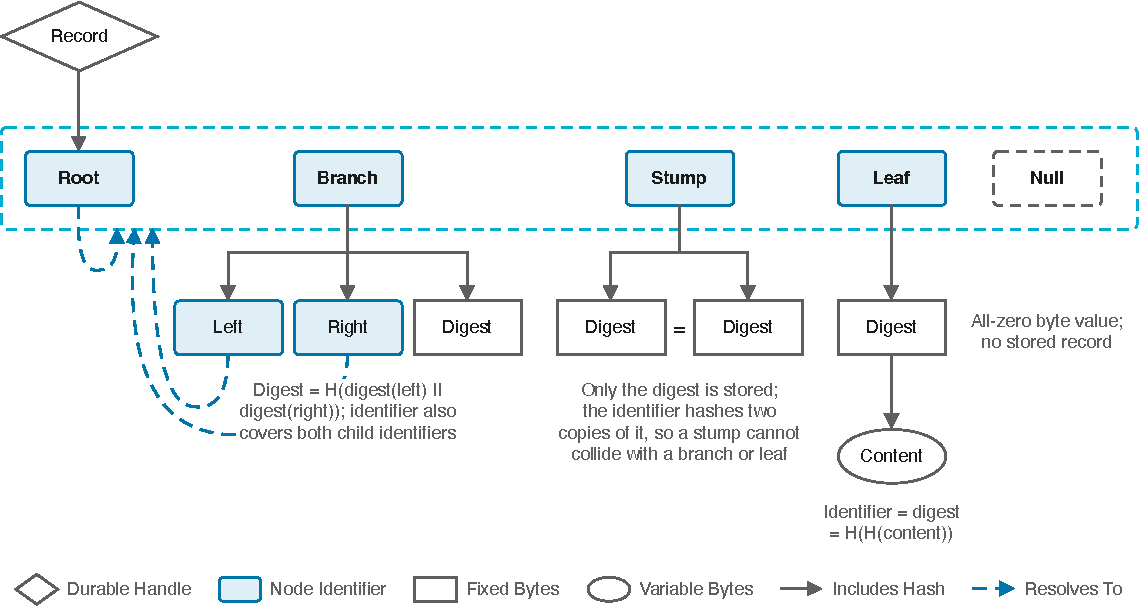
\includegraphics[scale=0.851]{figures/dag-stump.pdf}
  \caption{Roots and Partial State}
  \label{fig:dag-stump}
\end{figure}

\subsection{Proof Under Partial Knowledge}
\label{sec:partial-knowledge-proof}

The stump gives missing structure a precise place in this model by preserving the digest expected at one position and ending traversal at an identified boundary. Two states must remain distinct: null records actual emptiness, and a stump records committed structure awaiting evidence. A read that reaches a stump therefore returns a distinguished unknown value and makes no claim about what lies beneath. Partial knowledge is thus a precise statement about which regions of one immutable state are currently known.

Three operations move a state between levels of knowledge without changing its identity: slicing and pruning reduce the retained evidence, and merging restores missing evidence. A \glslink{slice}{slice} follows selected semantic \glslink{path}{paths} through a complete state and replaces unrelated material with stumps. Because the result retains the original root digest, every included resource remains bound to the complete state from which it came. Object-aware slicing follows compatible documented protocols as well as physical DAG edges. Object code may guide that traversal, but it is never trusted to preserve integrity, since the recipient verifies the resulting root against its accepted commitment. Slicing thereby extends the economy of compact Merkle multiproofs~\cite{Ramabaja2020compact}. A \glslink{journal}{journal} can apply the same stump replacement to material it already holds. \glslink{prune}{Pruning} shrinks what the journal retains and leaves the logical state, including every digest, unchanged. \glslink{merge}{Merge} moves in the other direction by replacing a stump with matching structure or recursively combining compatible branches. A digest mismatch aborts the operation, since the substrate cannot know which version a domain would prefer, and conflict resolution remains a matter of domain policy.

Partial states must also cross transport boundaries, and serialization carries node kinds, bytes, and retained digests between journals. A client can therefore reconstruct the same logical root, retain one proof, and accumulate neighboring evidence through later responses. \Cref{alg:deep-slice,alg:deep-prune,alg:merge-partial} give the slice, prune, and merge procedures. Each procedure evaluates the object it traverses (\cref{sec:objects}) and calls that object's operations.\footnote{Following Scheme convention, a name ending in \texttt{!} denotes an operation that modifies its target.}

\begin{algorithm}[htbp]
\caption{Deep Slice Along Object Path}
\label{alg:deep-slice}
\begin{algorithmic}[1]
\Require Object $x$ implementing digest-preserving slice/set protocols; nonempty available path $p$
\Ensure The selected path remains available and the logical digest remains fixed
\Function{DeepSlice}{$x,p$}
  \State $o \gets \texttt{sync-eval}(x)$
  \State $k \gets \Call{First}{p}$
  \If{$|p| = 1$}
    \State $o.\texttt{slice!}(k)$
    \State \Return $\Call{Node}{o}$
  \EndIf
  \State $c \gets o.\texttt{get}(k)$
  \State $d \gets \Call{Digest}{c}$
  \State $q \gets \Call{Rest}{p}$
  \State $c' \gets \Call{DeepSlice}{c,q}$
  \If{$\Call{Digest}{c'} \ne d$}
    \State \Call{Fail}{``slice changed child digest''}
  \EndIf
  \State $o.\texttt{set!}(k,c')$
  \State $o.\texttt{slice!}(k)$ \Comment{Discard siblings not needed for $k$.}
  \State \Return $\Call{Node}{o}$
\EndFunction
\end{algorithmic}
\end{algorithm}


\begin{algorithm}[htbp]
\caption{Deep Prune Along Object Path}
\label{alg:deep-prune}
\begin{algorithmic}[1]
\Require Object $x$ implementing digest-preserving prune/set protocols; nonempty path $p$ (may cross stumps)
\Ensure Evidence at the selected path is removed while the logical digest remains fixed
\Function{DeepPrune}{$x,p$}
  \State $o \gets \texttt{sync-eval}(x)$
  \State $k \gets \Call{First}{p}$
  \If{$|p| = 1$}
    \State $o.\texttt{prune!}(k)$
    \State \Return $\Call{Node}{o}$
  \EndIf
  \State $c \gets o.\texttt{get}(k)$
  \If{$c$ is not an available branch}
    \State \Return $\Call{Node}{o}$
  \EndIf
  \State $d \gets \Call{Digest}{c}$
  \State $q \gets \Call{Rest}{p}$
  \State $c' \gets \Call{DeepPrune}{c,q}$
  \If{$\Call{Digest}{c'} \ne d$}
    \State \Call{Fail}{``prune changed child digest''}
  \EndIf
  \If{$c'$ is a stump}
    \State $o.\texttt{prune!}(k)$
  \Else
    \State $o.\texttt{set!}(k,c')$
  \EndIf
  \State \Return $\Call{Node}{o}$
\EndFunction
\end{algorithmic}
\end{algorithm}


\begin{algorithm}[htbp]
\caption{Deep Merge of Compatible Structures}
\label{alg:merge-partial}
\begin{algorithmic}[1]
\Require Partial structures $a$ and $b$
\Ensure The result contains the union of available evidence and retains the common digest
\Function{MergePartial}{$a,b$}
  \If{$\Call{Digest}{a} \ne \Call{Digest}{b}$}
    \State \Call{Fail}{``cannot merge different digests''}
  \EndIf
  \If{$a$ is null}
    \State \Return $a$
  \ElsIf{$a$ is a leaf}
    \State \Return $a$
  \ElsIf{$a$ is a stump}
    \State \Return $b$
  \ElsIf{$b$ is a stump}
    \State \Return $a$
  \Else
    \State $a_L \gets \Call{Left}{a}$; $b_L \gets \Call{Left}{b}$
    \State $a_R \gets \Call{Right}{a}$; $b_R \gets \Call{Right}{b}$
    \State $l \gets \Call{MergePartial}{a_L,b_L}$
    \State $r \gets \Call{MergePartial}{a_R,b_R}$
    \State \Return $\Call{Branch}{l,r}$
  \EndIf
\EndFunction
\end{algorithmic}
\end{algorithm}


\subsection{Integrity as Infrastructure}

Partial knowledge separates auditability from bulk custody. An auditor need retain only the report, definitions, path, and ancestor evidence relevant to one decision, while the source keeps operational data in its native system. Another institution may preserve a complementary slice, and the two copies remain comparable because both resolve to the same commitment. Integrity does not, however, guarantee availability, which depends on institutions that replicate, \glslink{pin}{pin}, and renew media. A digest may outlive every full copy of the bytes it names. Integrity lets anyone check a recovered copy, but only retention determines whether recovery remains possible. When parties with different interests and storage budgets share these responsibilities, each can transfer, cite, sample, or inspect only the material it needs. The substrate is kept deliberately small because it concentrates trust, and everything above it is meaningful only if its primitives are correct. Rich semantics stay above it in stored objects, where they remain visible and can evolve historically. Structural validity alone is not a sufficient defense, since well-formed evidence may still be adversarially deep or broad; verification therefore also bounds how large, deep, and expensive an accepted proof may be. Within those bounds, the substrate adds verifiable internal partiality to content addressing, so that structure can be selectively retained and later restored under one identity. Signed committed \glslink{step}{steps} then extend that identity across change.
